\chapter{System testing and evaluation}

\FloatBarrier

\section{Evaluation questions and evidence organization}

Evaluation addresses the four questions introduced at the beginning of the thesis. Functional tests examine whether stock changes are bounded and attributed. Concurrency and replay tests examine whether repeated or competing intentions produce acceptable results. Warning tests examine the separation of severity, recovery and review. Browser checks examine presentation and navigation. Local measurements and recorded failure scenarios examine the optional cache path and durable state.


The evidence has several dates and purposes. The backend and frontend result images included here are from 5 October 2026. The original browser acceptance record and performance and recovery records are dated 3 October UTC, corresponding to the local development session that produced them. A later capture run on 5 October obtains the expanded interface collection without posting new business data. These records are not interchangeable samples of one experiment.


\begingroup\small\setstretch{1.05}\setlength{\tabcolsep}{3pt}\renewcommand{\arraystretch}{1.25}
\begin{longtable}{>{\raggedright\arraybackslash}p{0.3\textwidth}>{\raggedright\arraybackslash}p{0.3\textwidth}>{\raggedright\arraybackslash}p{0.3\textwidth}}
\caption{Evaluation evidence and its scope}\label{tab:evidence-dates}\\
\toprule
\textbf{Evidence} & \textbf{Recorded date} & \textbf{What it establishes} \\
\midrule\endfirsthead
\toprule
\textbf{Evidence} & \textbf{Recorded date} & \textbf{What it establishes} \\
\midrule\endhead
\bottomrule\endfoot
Backend result log & 5 October 2026 local time & Twenty-seven integration cases completed without failures \\
Frontend result log & 5 October 2026 local time & Three threshold presentation tests passed \\
Original browser journey & 3 October 2026 UTC & Fourteen checks including one receipt and one acknowledgement \\
Expanded figure capture & 5 October 2026 UTC & Twenty-seven captures role guard checks and no page runtime errors \\
Warning-query benchmark & 3 October 2026 UTC & Six hundred sequential measured samples per mode \\
Redis interruption & 3 October 2026 UTC & Equivalent warning result during the recorded cache outage \\
Restart fingerprint & Preserved repository record & Equal selected product and transaction rows after restart \\
\end{longtable}\endgroup

The prototype uses fictitious records and local services. Tests can provide strong evidence for a specified invariant while still leaving practical questions unanswered. In particular, the study does not measure store-user learning, business losses avoided, supplier lead times or production capacity. The result discussion keeps the units and scope of each claim aligned with the recorded procedure.


\FloatBarrier

\section{Backend integration testing}

\FloatBarrier

\subsection{Environment and case coverage}

The backend test class uses Testcontainers to create MySQL and Redis instances for the test execution. Its dynamic properties direct the Spring application to those instances. This is valuable because locking, uniqueness and persistence behavior involve the actual database rather than an in-memory substitute. It does not mean that every production database setting or fault mode is reproduced.


The current integration suite contains 46 cases covering authentication, CSRF, role restrictions, catalogue validation, quantity changes, audit history, retry behavior, concurrency, shortage transitions, batch allocation, expiry policy, slow-moving detection, purchase approval, partial receipts, stock reviews and account safeguards. The result in Figure~\ref{fig:backend-result} reports zero failures, errors and skipped tests for the recorded run. A passing suite means that those executable assertions held in this run. It is not a numerical code-coverage percentage or a proof that all possible requests are correct.


\begin{figure}[htbp]\centering
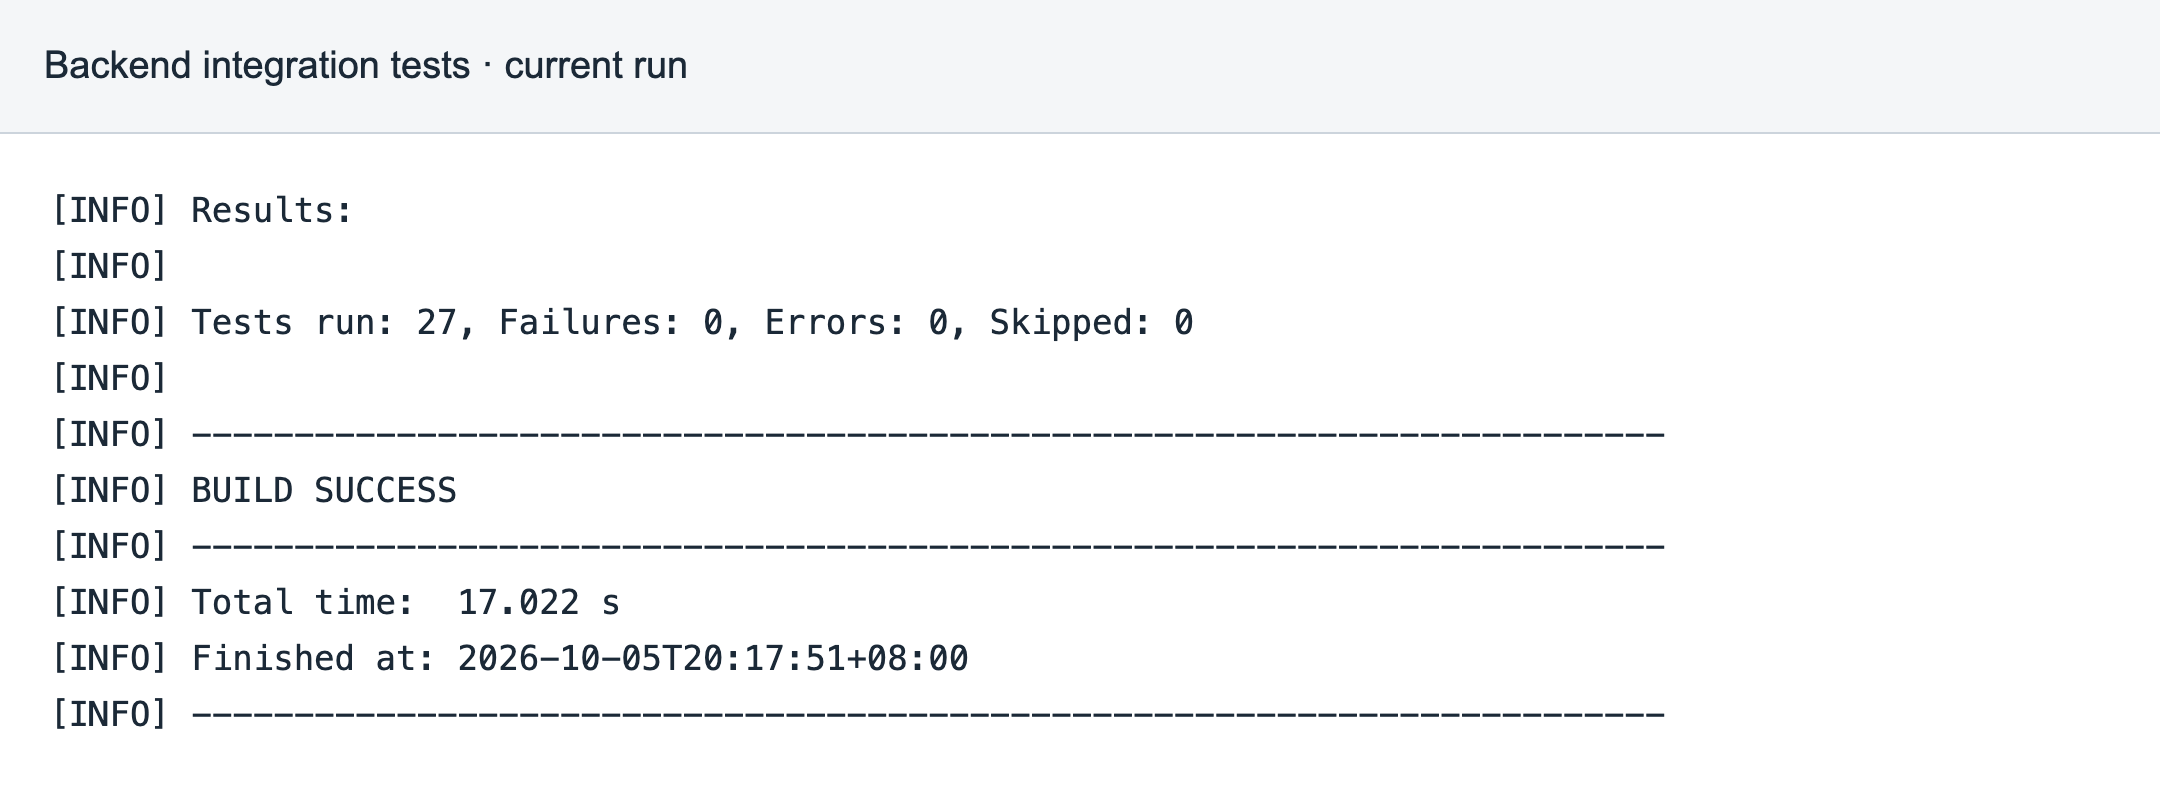
\includegraphics[width=\textwidth,height=0.40\textheight,keepaspectratio]{../figure-assets/evidence/01-backend-tests.png}
\caption{Backend integration result from the 5 October 2026 execution}\label{fig:backend-result}
\end{figure}

\begingroup\small\setstretch{1.05}\setlength{\tabcolsep}{3pt}\renewcommand{\arraystretch}{1.25}
\begin{longtable}{>{\raggedright\arraybackslash}p{0.3\textwidth}>{\raggedright\arraybackslash}p{0.3\textwidth}>{\raggedright\arraybackslash}p{0.3\textwidth}}
\caption{Main backend acceptance groups}\label{tab:backend-groups}\\
\toprule
\textbf{Group} & \textbf{Representative assertions} & \textbf{Reported outcome} \\
\midrule\endfirsthead
\toprule
\textbf{Group} & \textbf{Representative assertions} & \textbf{Reported outcome} \\
\midrule\endhead
\bottomrule\endfoot
Authentication & Anonymous denial invalid credentials and missing login fields & Passed \\
Authorization & Clerk review denial manager posting denial and threshold boundary & Passed \\
Catalogue & Unique SKU valid threshold hierarchy and archived movement denial & Passed \\
Stock arithmetic & Receipt dispatch signed adjustment absolute count and zero count & Passed \\
Audit behavior & Before and after history and unchanged stocktake observation & Passed \\
Retries & Equal replay identifier and changed-payload conflict & Passed \\
Concurrency & No overselling identical submission and first reviewer preservation & Passed \\
Warnings & Zero equality healthy recovery severity renewal and accurate filters & Passed \\
Administration & Last enabled administrator cannot be disabled or demoted & Passed \\
\end{longtable}\endgroup

\FloatBarrier

\subsection{Negative-stock and audit consistency}

The insufficient-stock test attempts a dispatch from an empty product. It expects a domain exception, unchanged transaction count and unchanged quantity. This checks both the arithmetic boundary and the absence of an accepted history row for a rejected operation. The receipt-and-dispatch test then verifies a valid sequence: before zero, receipt eight, dispatch three and final quantity five with two movements.


The absolute-count cases verify the semantic distinction from a relative adjustment. Starting at ten, an adjustment of negative two produces eight; counting three then produces delta negative five and after quantity three. Counting to zero is also accepted and auditable. An unchanged count creates a zero-delta history row. These cases would not be equivalent to a generic test that an input number can be stored in a product field.


\FloatBarrier

\subsection{Duplicate and concurrent requests}

The exact-replay case sends the same actor-scoped request twice and checks the same movement identifier and one stock effect. A changed quantity with that key produces a conflict. These assertions connect the returned response to the stored result rather than merely checking that the server returns a success status.


The concurrency source in Figure~\ref{fig:concurrency-code} shows two demanding scenarios. Twelve unit dispatch attempts compete for a starting balance of seven; the test expects exactly seven successes and quantity zero. Four concurrent identical stock-in submissions must produce one identifier and quantity four. Those bounds directly test the intended outcome under the selected same-product workload.


\begin{figure}[htbp]\centering
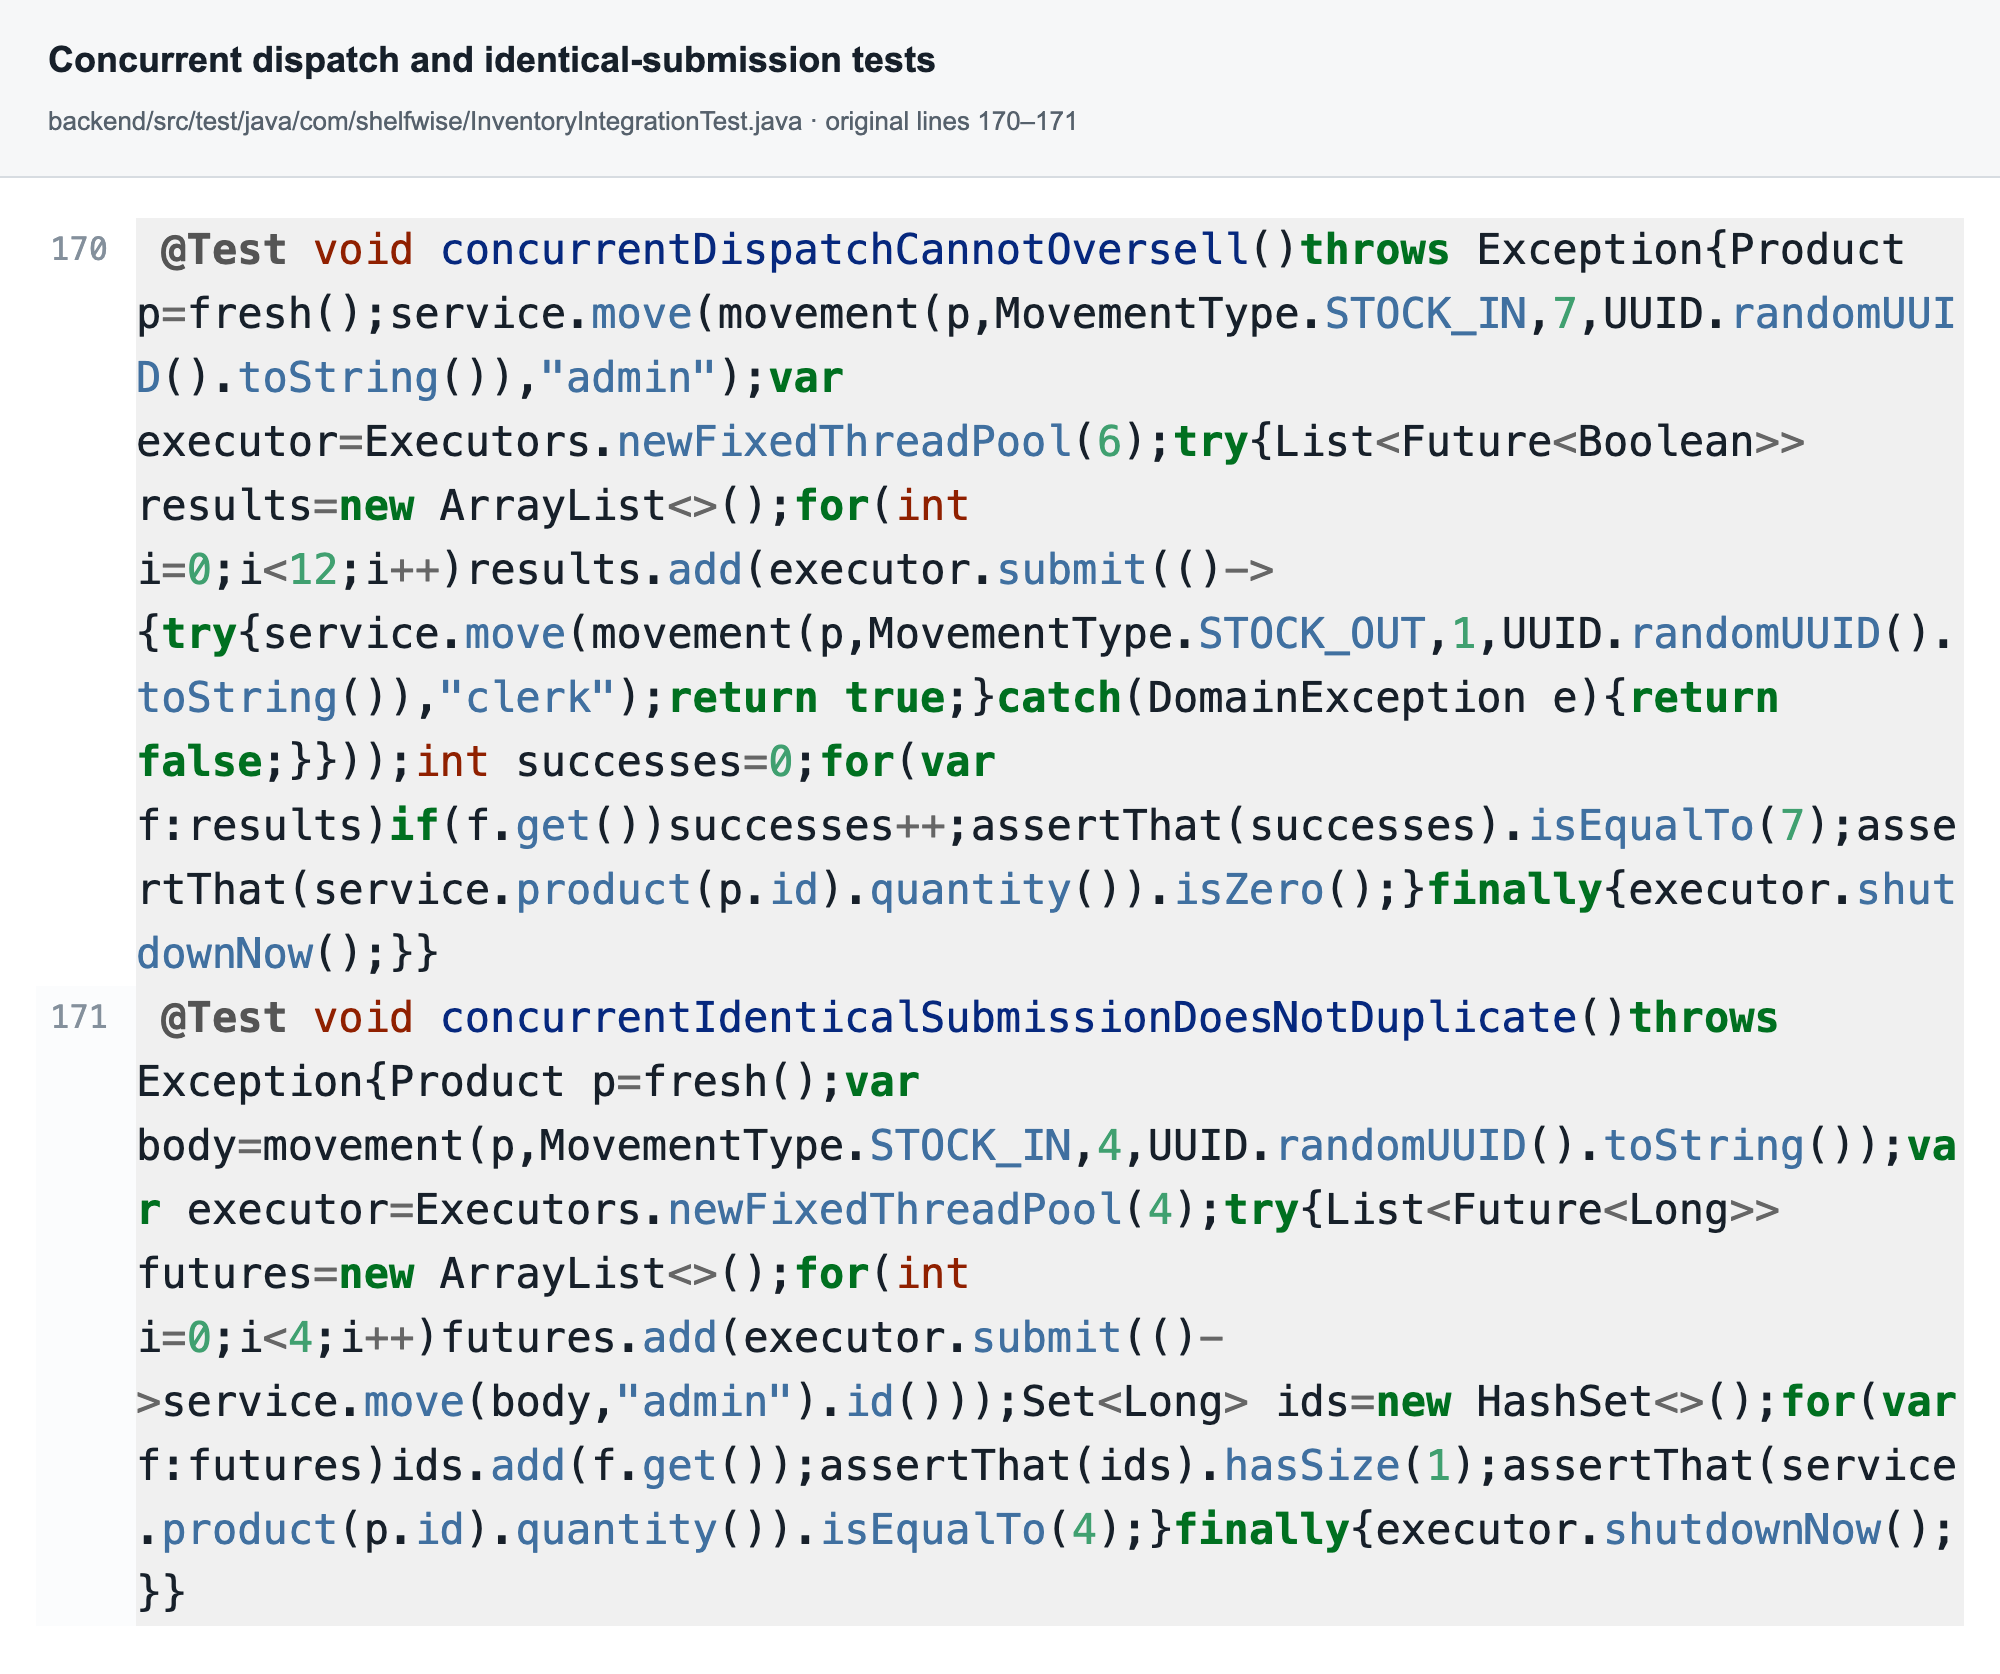
\includegraphics[width=\textwidth,height=0.84\textheight,keepaspectratio]{../figure-assets/code/12-code-concurrency-tests.png}
\caption{Actual concurrent dispatch and identical-submission integration cases}\label{fig:concurrency-code}
\end{figure}

The tests do not establish fairness, sustained throughput or behavior under every lock timeout. The shared revision row can serialize parts of writes across different products. Cross-product reuse of one actor-key pair and database deadlocks require additional targeted cases. MySQL's documentation treats deadlocks as a transaction condition that applications must consider \citep{mysql-deadlocks}; the current service does not advertise an automatic deadlock-retry policy.


\FloatBarrier

\subsection{Warning and review assertions}

The threshold test verifies OUT at zero and LOW at exact positive equality. Healthy replenishment removes the active shortage and creates RESTOCKED. Expiry tests verify the inclusive expiry-day boundary under the configured timezone, and slow-moving tests verify that sales-only history forms one continuous event. A review test verifies that acknowledgement becomes visible through the cache and leaves quantity zero. The concurrent-review case expects both responses to expose the same first reviewer. Archive cases confirm that the product rejects movements and its open warnings are resolved.


The recovery test named for restocked expiry and new shortage exercises renewed shortage after replenishment. Separate expiry tests exercise business-day boundaries, invalid timezone rejection and expiry-aware sellable balances. They do not establish a long-running scheduler reliability distribution. The supported conclusion is that the implemented rules agree at the tested boundaries; broader clock, cache and operational scheduling workloads remain future work.


\FloatBarrier

\section{Batch, purchasing and review workflow testing}

The expanded backend cases exercise receipt metadata replay, concurrent receipts, FEFO/FIFO batch allocation, exclusion of expired or quarantined batches, and disposal approval after a batch remainder changes. These assertions connect physical stock to sellable stock rather than checking only a product-level integer.


Purchase tests cover multi-line draft creation, rejection and edit, completion, partial receipt, receipt replay, cancellation and concurrent approval. Approval rechecks the current replenishment suggestion before accepting a quantity. A receipt is therefore both a purchasing event and an audited stock movement; replay must not create a second batch or movement.


Stock-review tests cover count and disposal submissions, stale snapshots, idempotent submissions, long bounded reasons and role denials. The approval path applies a movement only after the stored snapshot or batch remainder is still valid. These cases are stronger evidence for the expanded workflow than a screenshot of a review button, but they remain synthetic single-store scenarios.


\FloatBarrier

\section{Frontend and browser testing}

\FloatBarrier

\subsection{Threshold presentation}

The frontend unit tests check the zero boundary, exact threshold equality and positive healthy stock. The source in Figure~\ref{fig:frontend-test-code} makes those values visible. The result in Figure~\ref{fig:frontend-result} confirms three passing cases. The tests protect the labels shown beside quantity so that the browser does not contradict the server's fundamental classification.


\begin{figure}[htbp]\centering
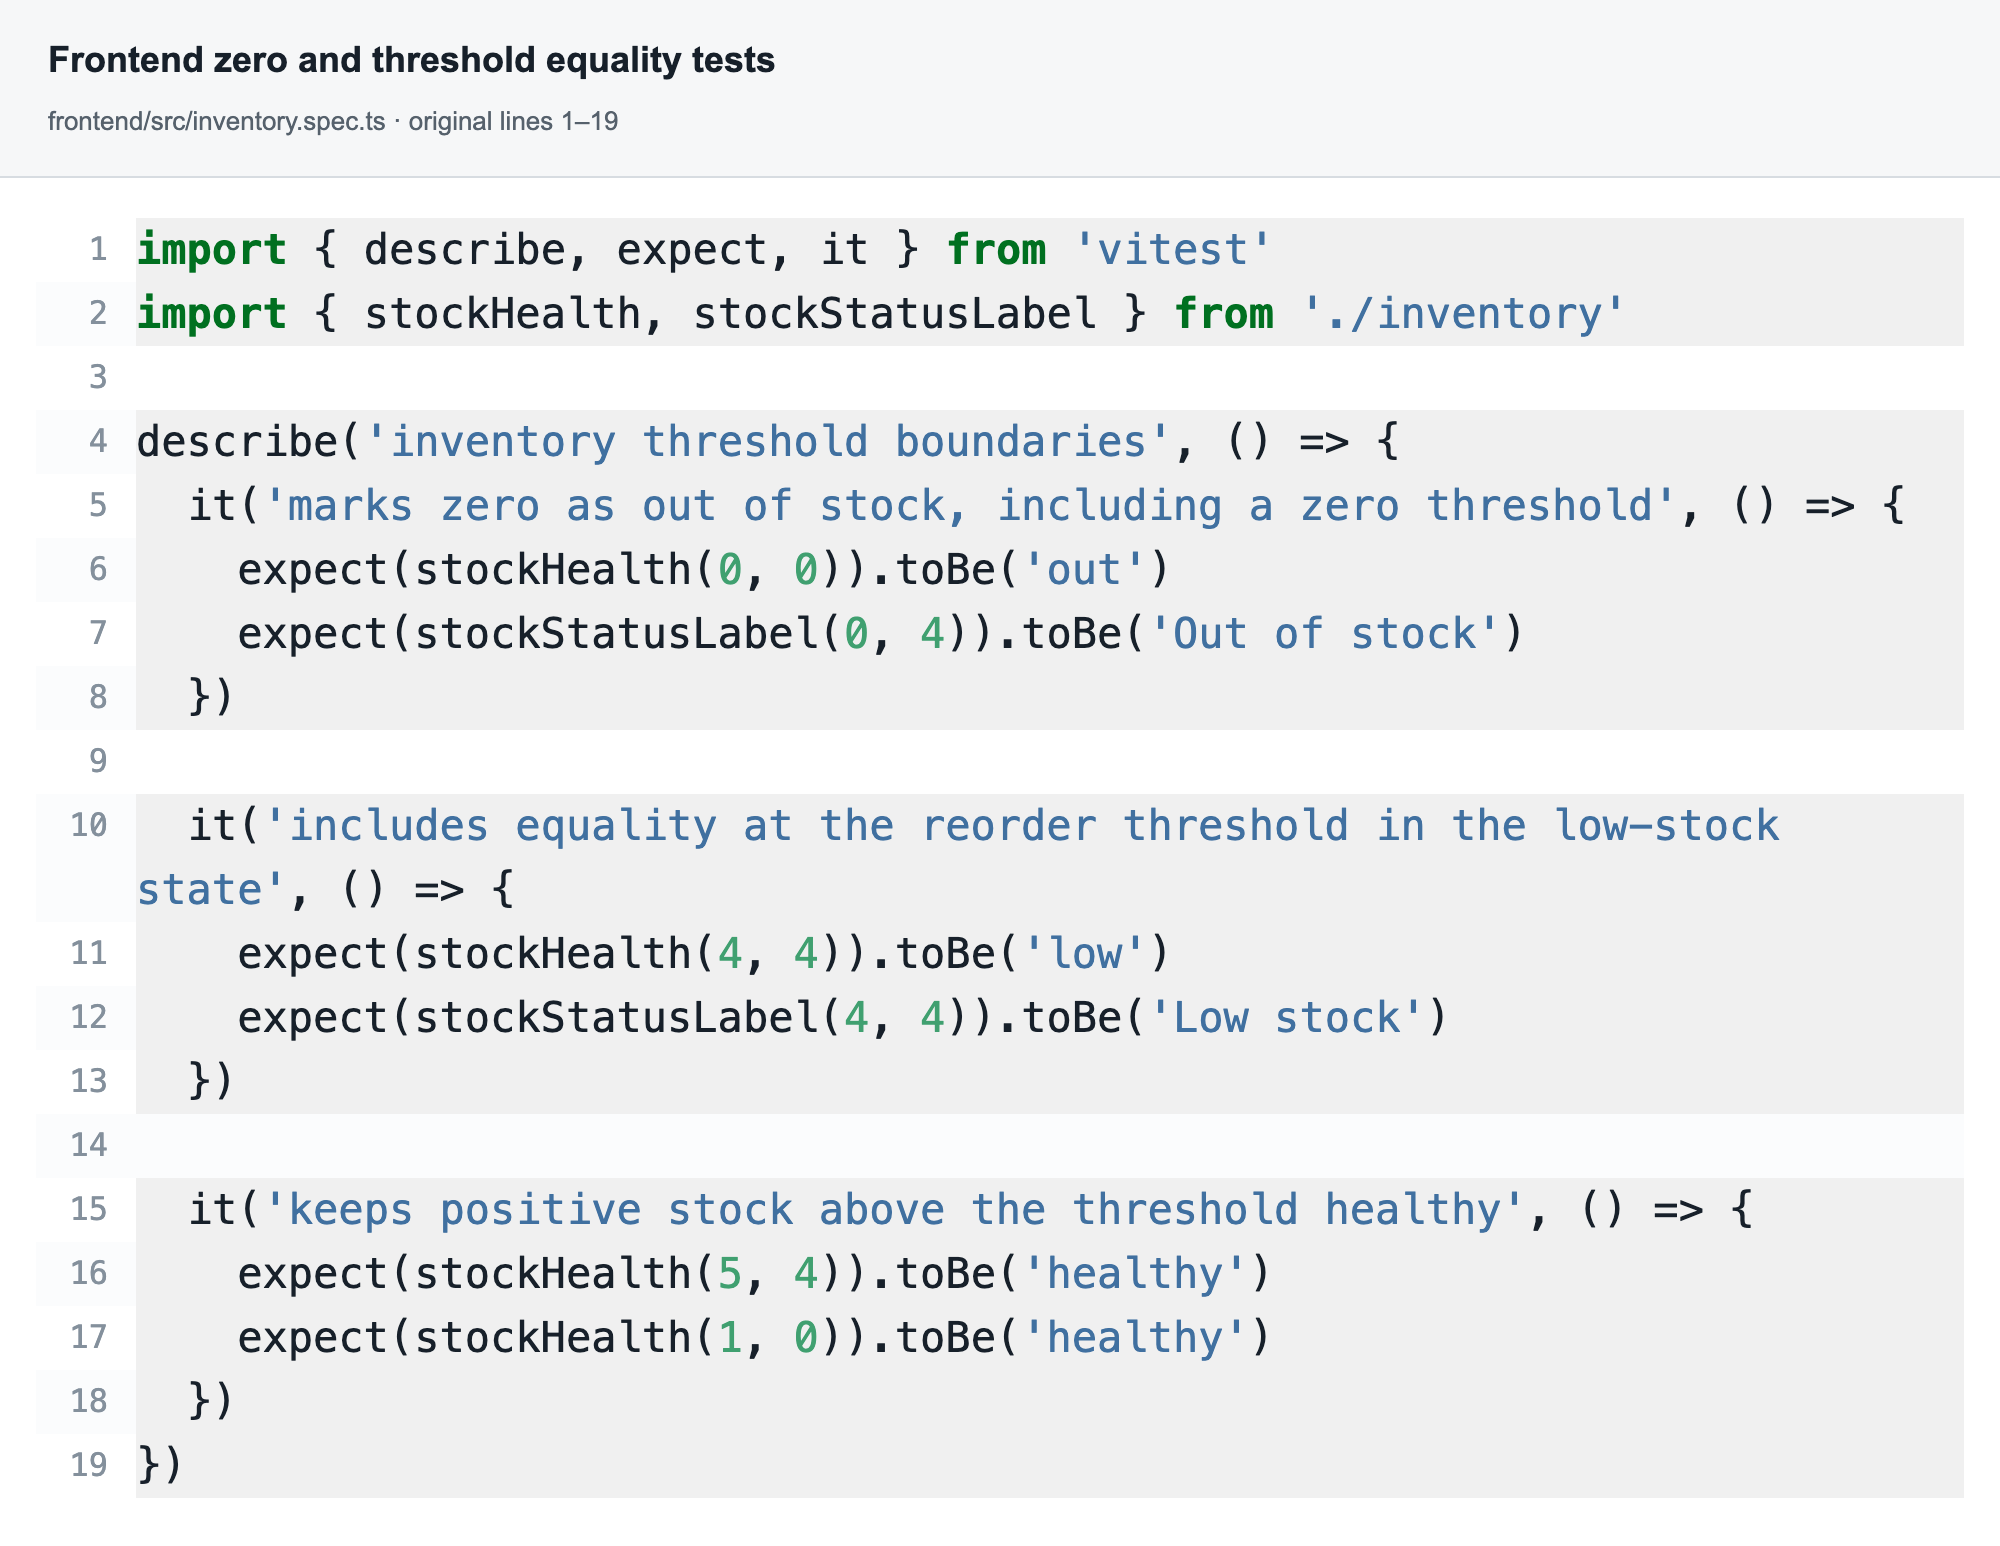
\includegraphics[width=\textwidth,height=0.84\textheight,keepaspectratio]{../figure-assets/code/13-code-boundary-tests.png}
\caption{Frontend test inputs for zero equality and healthy stock}\label{fig:frontend-test-code}
\end{figure}

\begin{figure}[htbp]\centering
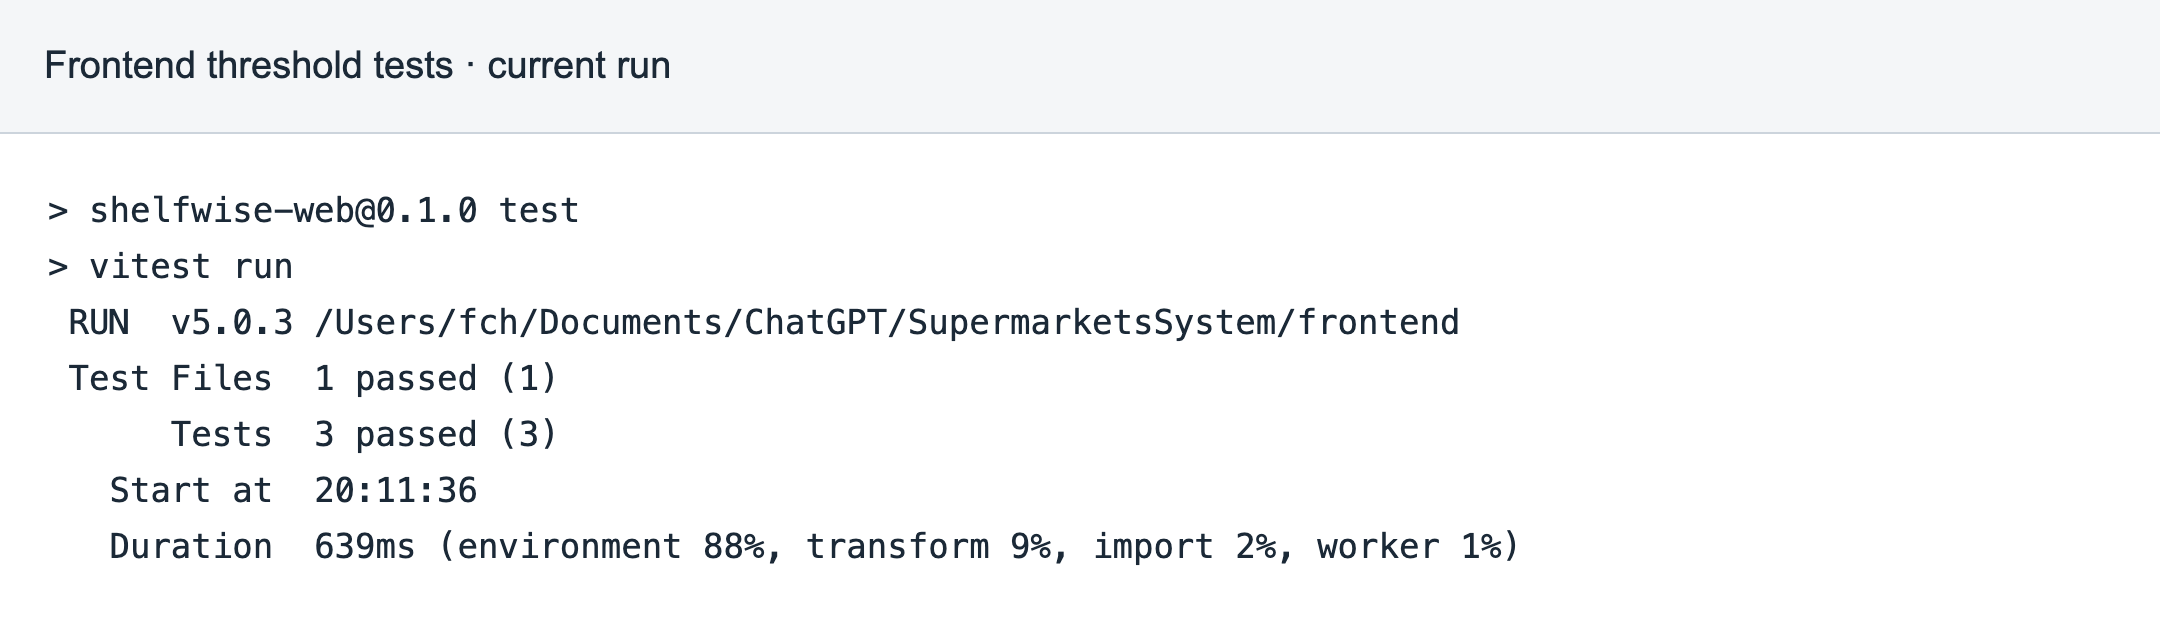
\includegraphics[width=\textwidth,height=0.40\textheight,keepaspectratio]{../figure-assets/evidence/02-frontend-tests.png}
\caption{Frontend unit-test result from the current execution}\label{fig:frontend-result}
\end{figure}

These are small focused tests. They do not cover every modal, asynchronous loading state or component interaction. The broader browser journeys serve a complementary purpose by opening the application and observing rendered behavior. Neither layer establishes full accessibility conformance or practical usability for store employees.


\FloatBarrier

\subsection{Earlier operational browser journey}

The preserved earlier browser record contains fourteen checks with zero JavaScript runtime errors. It covers administrator login and operational views, an empty search, an actual receipt submission with the correct delta, clerk and manager navigation restrictions, managerial acknowledgement and phone-sized viewport containment. Its write operations make it stronger evidence of an interface-to-server journey than a collection of screenshots alone.


The empty-result interface in Figure~\ref{fig:empty-ui} illustrates the recovery state used by the search check. It presents an explanation and a way to clear filters. A successful empty selection should not be confused with a failed request; error handling and query results represent different conditions in the application.


\begin{figure}[htbp]\centering
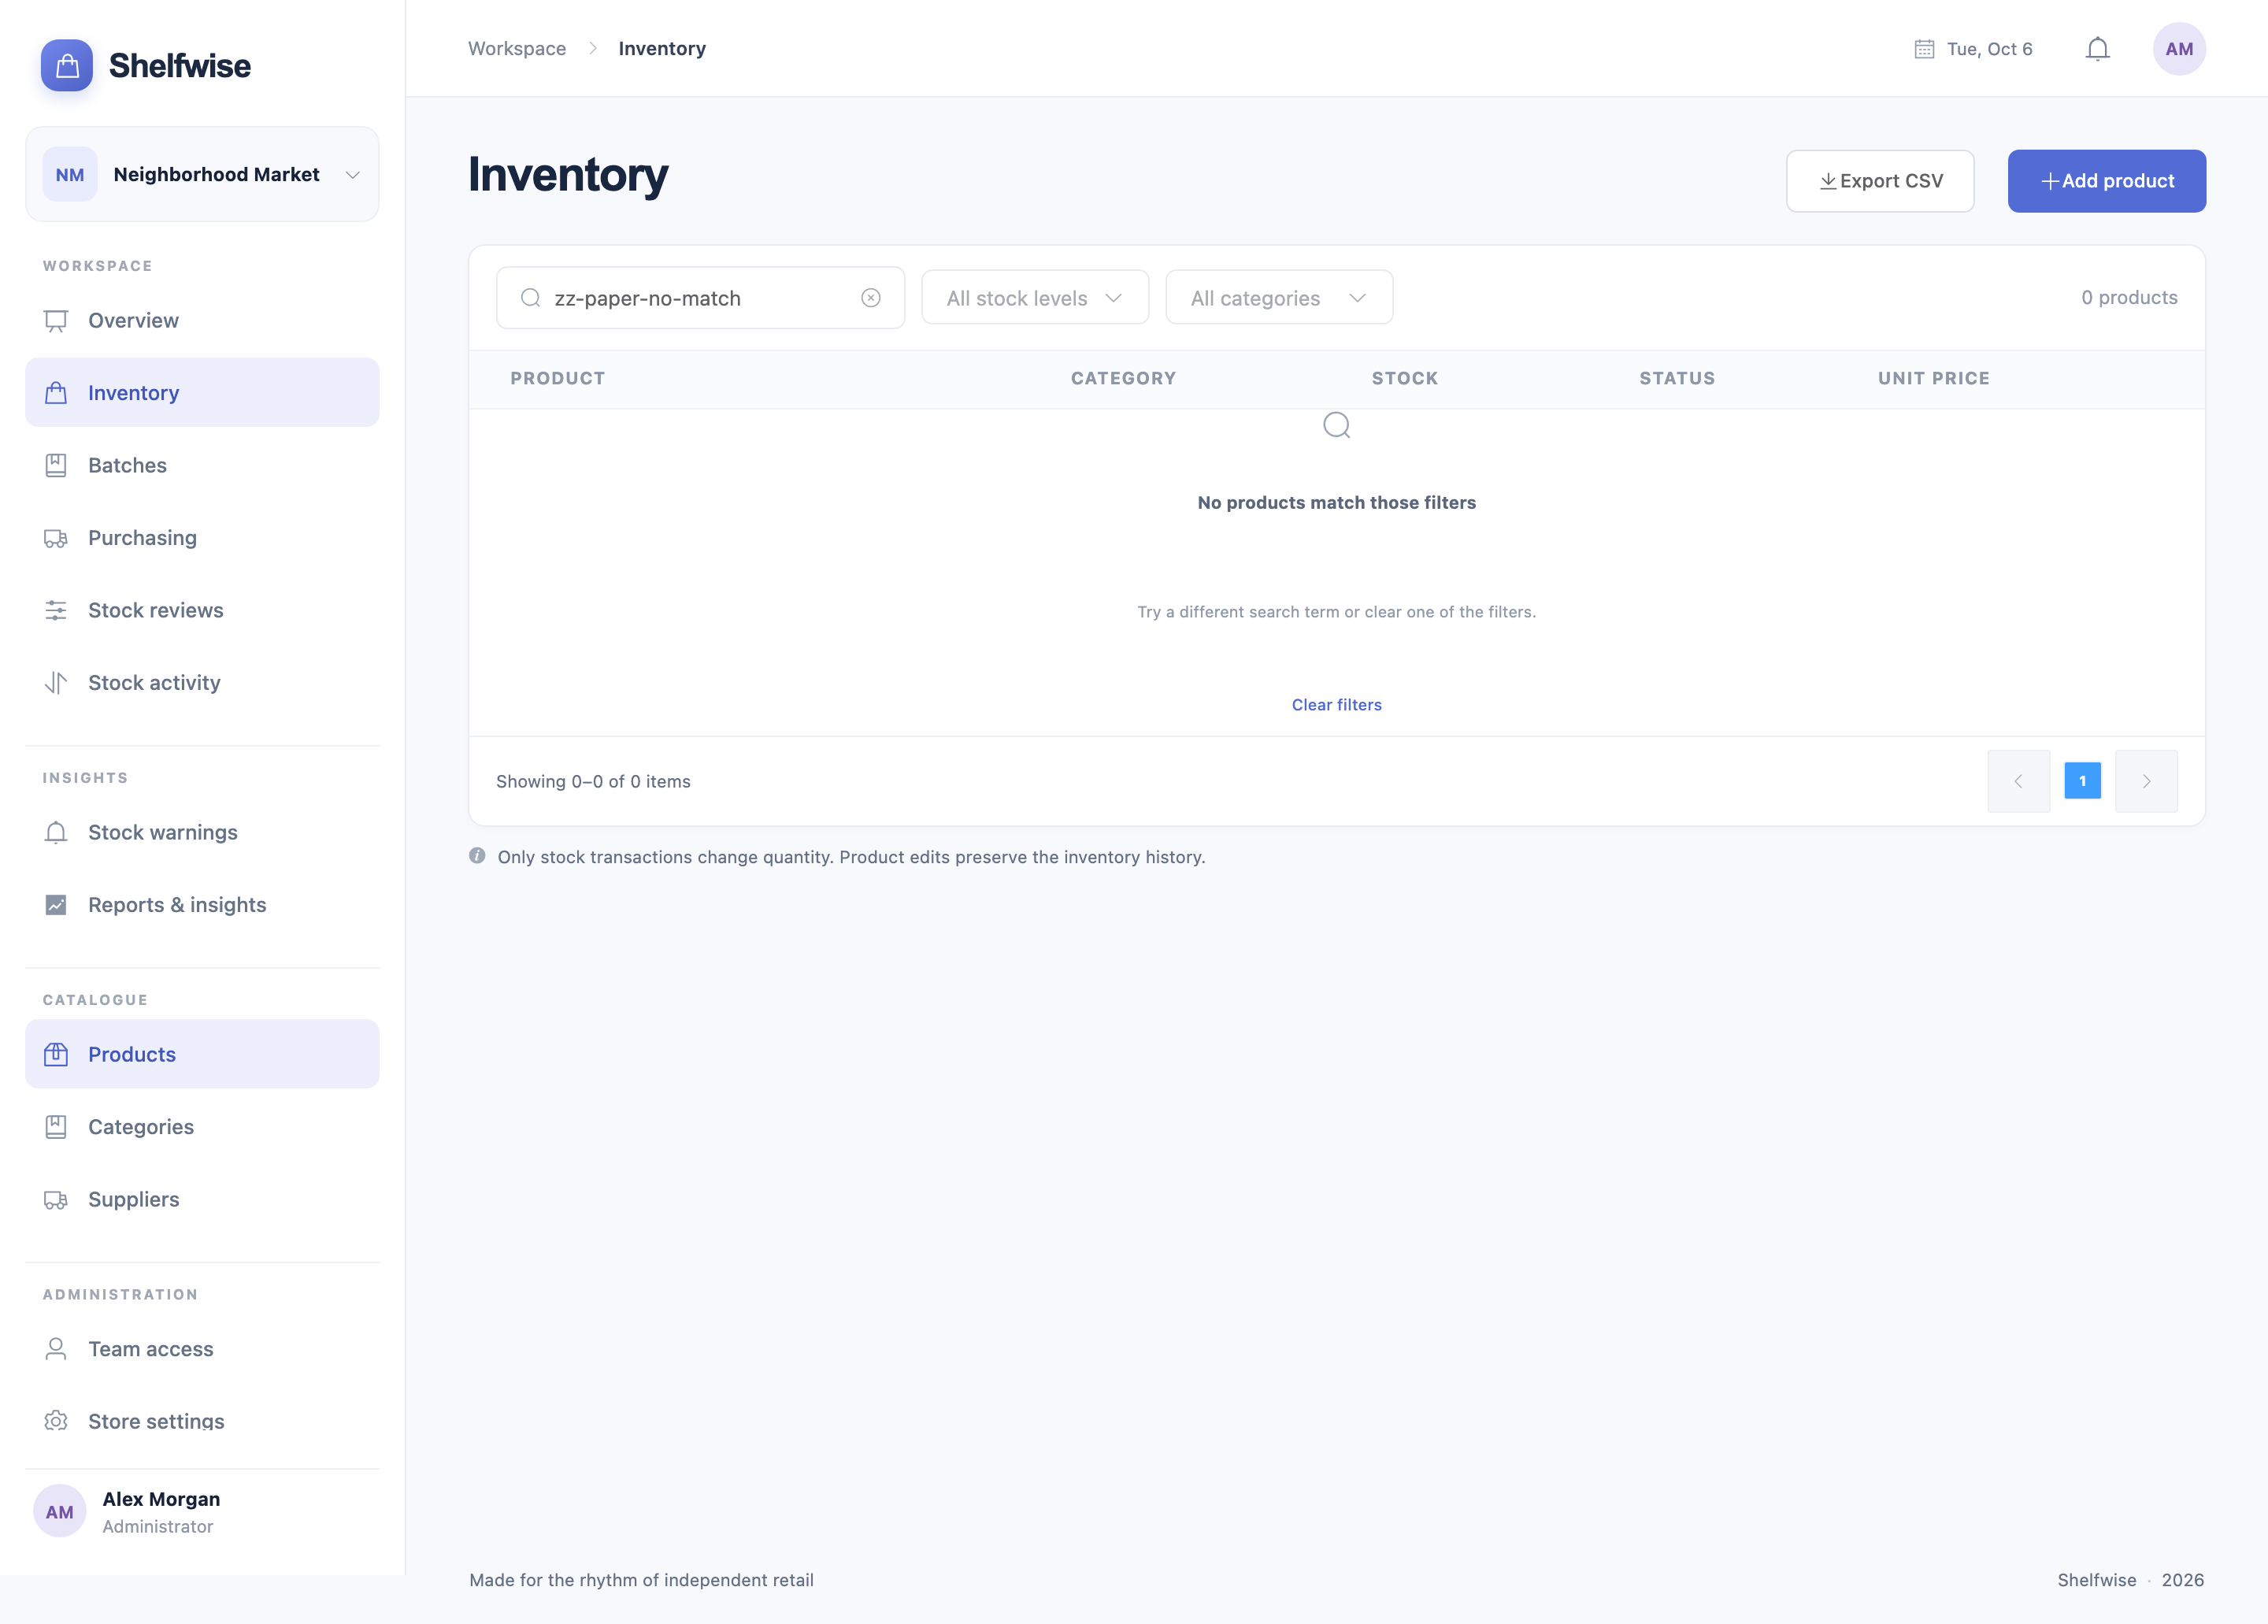
\includegraphics[width=\textwidth,height=0.40\textheight,keepaspectratio]{../figure-assets/ui/13-empty-search.png}
\caption{Empty inventory search with a visible recovery action}\label{fig:empty-ui}
\end{figure}

\FloatBarrier

\subsection{Expanded capture verification}

The later capture run obtains twenty-seven interfaces and forms. It signs in as all three roles, checks that managers cannot reach staff administration and clerks cannot reach the warning board, and checks document width at 390 pixels. It records zero page runtime errors. The verification image in Figure~\ref{fig:browser-result} identifies this capture-specific evidence.


\begin{figure}[htbp]\centering
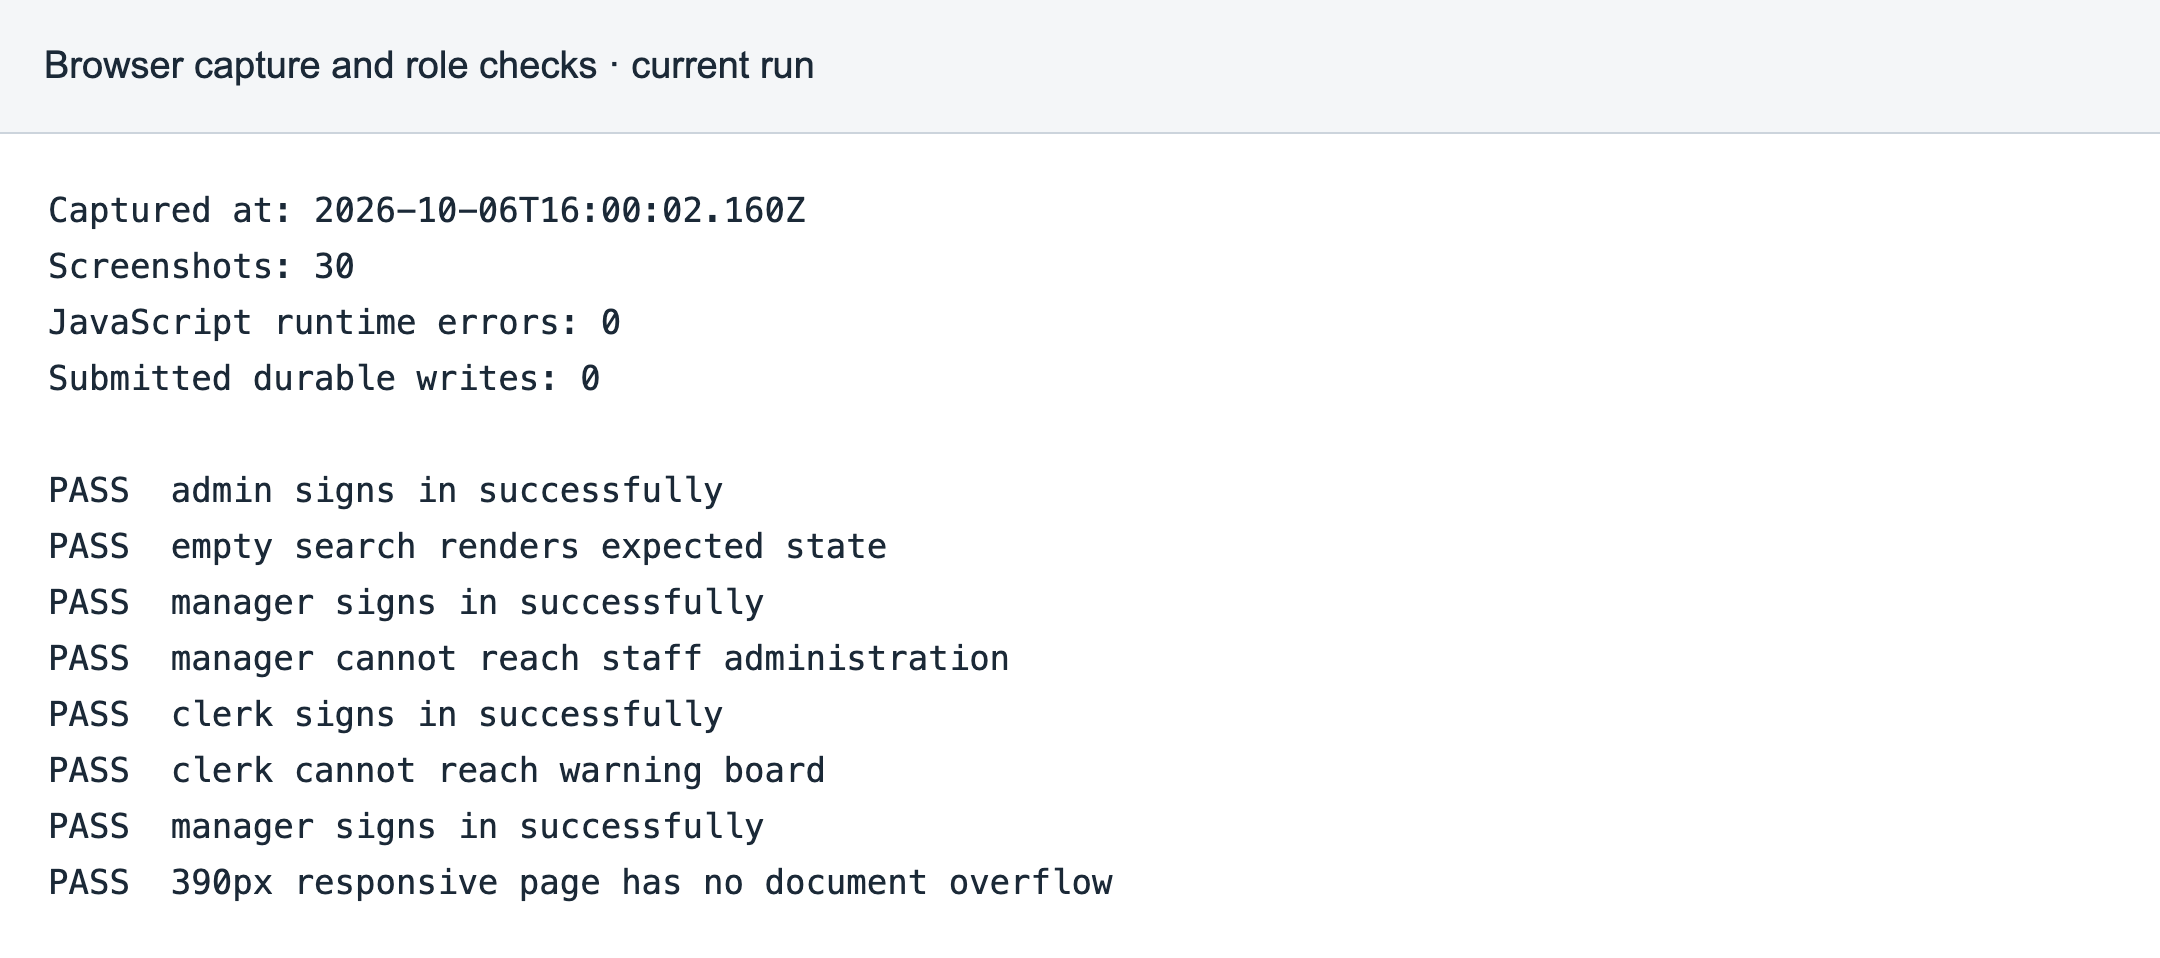
\includegraphics[width=\textwidth,height=0.40\textheight,keepaspectratio]{../figure-assets/evidence/03-browser-verification.png}
\caption{Capture-run checks and the absence of posted business changes}\label{fig:browser-result}
\end{figure}

The capture process opens forms and fills drafts but does not submit stock, account or catalogue changes. Receipt and dispatch images therefore demonstrate the implemented controls and labels, not additional accepted movements. The thesis uses the earlier operational journey and backend cases when discussing accepted writes. This separation allows screenshots to remain useful without assigning them evidential weight they do not have.


\FloatBarrier

\section{Performance test of the warning query}

\FloatBarrier

\subsection{Workload and measurement procedure}

The performance record compares the warning query with cache enabled and with cache bypassed. It uses sixteen products, sixteen open warning episodes, page size one hundred and concurrency one. Three rounds alternate the mode order. Each mode receives twenty warm-up requests and two hundred measured requests per round, giving six hundred measured samples for each mode. Results include the local HTTP path rather than isolated Redis or MySQL operation time.


The recorded host is Apple Silicon macOS with MySQL and Redis containers accessed over loopback. The script records the operating system, machine type, Python version and backend/database baseline. Authentication, durable revision retrieval, filtering, serialization and network handling can contribute to each response. A cache hit therefore avoids only part of the total request work.


\begingroup\small\setstretch{1.05}\setlength{\tabcolsep}{3pt}\renewcommand{\arraystretch}{1.25}
\begin{longtable}{>{\raggedright\arraybackslash}p{0.45\textwidth}>{\raggedright\arraybackslash}p{0.45\textwidth}}
\caption{Recorded local benchmark workload}\label{tab:benchmark-workload}\\
\toprule
\textbf{Parameter} & \textbf{Value} \\
\midrule\endfirsthead
\toprule
\textbf{Parameter} & \textbf{Value} \\
\midrule\endhead
\bottomrule\endfoot
Products & 16 \\
Open warning episodes & 16 \\
Page size & 100 \\
Concurrent requests & 1 \\
Alternating measurement rounds & 3 \\
Warm-up requests per mode per round & 20 \\
Measured requests per mode per round & 200 \\
Pooled measured samples per mode & 600 \\
Network and service placement & Loopback HTTP and local Colima containers \\
\end{longtable}\endgroup

The benchmark is preserved evidence, not a newly executed production experiment. The inclusion of warm-up and alternating order improves interpretability, but it does not remove all variation due to the host, containers or background activity. No simultaneous-user or capacity curve can be inferred from sequential requests.


\FloatBarrier

\subsection{Descriptive latency results}

The summary in Table~\ref{tab:latency} reports pooled median and tail percentiles from the preserved samples. Percentiles use the sorted-sample index implemented by the project's evaluation script. The Redis-enabled path has a median of approximately 5.33 ms, compared with approximately 6.56 ms for bypass. Its p95 is approximately 7.57 ms, compared with 8.11 ms. These are measurements in this particular run, not latency targets guaranteed by the architecture.


\begingroup\small\setstretch{1.05}\setlength{\tabcolsep}{3pt}\renewcommand{\arraystretch}{1.25}
\begin{longtable}{>{\raggedright\arraybackslash}p{0.18\textwidth}>{\raggedright\arraybackslash}p{0.18\textwidth}>{\raggedright\arraybackslash}p{0.18\textwidth}>{\raggedright\arraybackslash}p{0.18\textwidth}>{\raggedright\arraybackslash}p{0.18\textwidth}}
\caption{Warning-query latency from six hundred samples per mode}\label{tab:latency}\\
\toprule
\textbf{Mode} & \textbf{Samples} & \textbf{Median ms} & \textbf{p95 ms} & \textbf{p99 ms} \\
\midrule\endfirsthead
\toprule
\textbf{Mode} & \textbf{Samples} & \textbf{Median ms} & \textbf{p95 ms} & \textbf{p99 ms} \\
\midrule\endhead
\bottomrule\endfoot
Redis enabled & 600 & 5.33 & 7.57 & 8.87 \\
MySQL bypass & 600 & 6.56 & 8.11 & 9.42 \\
\end{longtable}\endgroup

The bar chart in Figure~\ref{fig:latency-summary} presents the same descriptive statistics. It helps separate the typical result from the upper-tail values. The approximately 1.24 ms difference between pooled medians is small in absolute terms. It is associated with the optional cache path under this dataset, while the benchmark includes costs that the cache cannot remove.


\begin{figure}[htbp]\centering
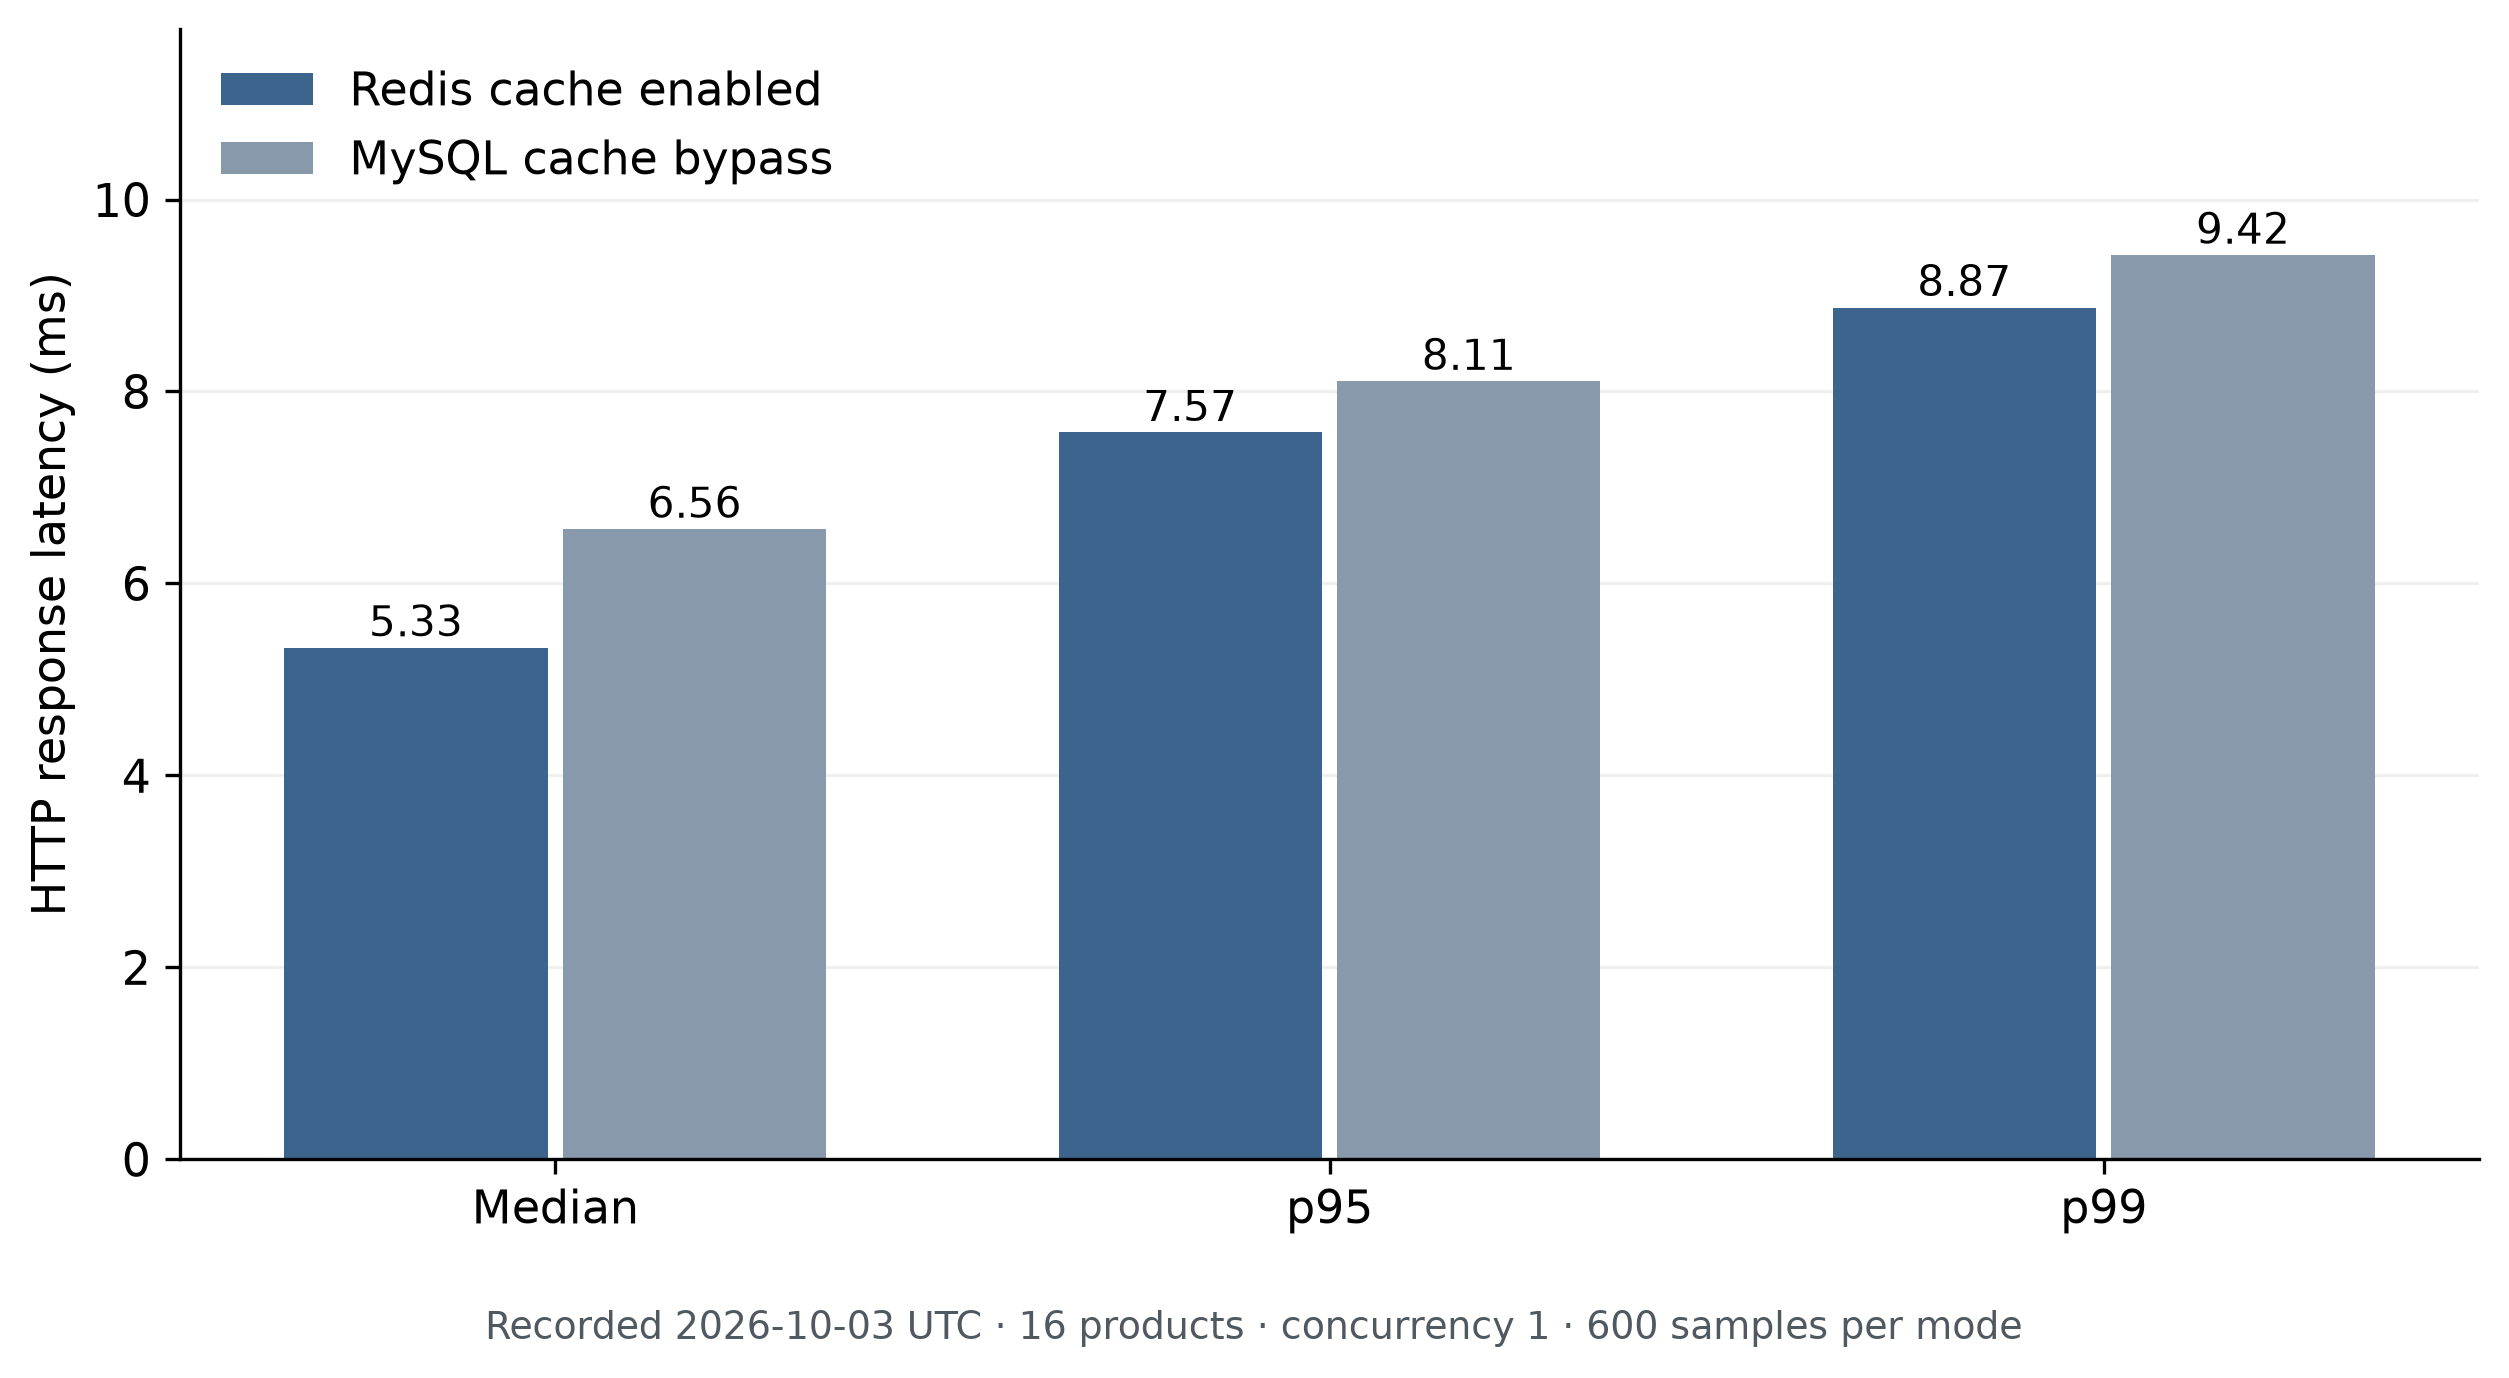
\includegraphics[width=\textwidth,height=0.40\textheight,keepaspectratio]{../figure-assets/evidence/04-latency-summary.png}
\caption{Pooled local median and tail latency for cached and bypass warning queries}\label{fig:latency-summary}
\end{figure}

The empirical cumulative distribution in Figure~\ref{fig:latency-ecdf} shows the proportion of measured responses below each latency. It reveals overlapping distributions instead of implying that every cached request is faster than every bypass request. The plotted tail also makes occasional slower observations visible. No statistical hypothesis test or confidence interval is reported.


\begin{figure}[htbp]\centering
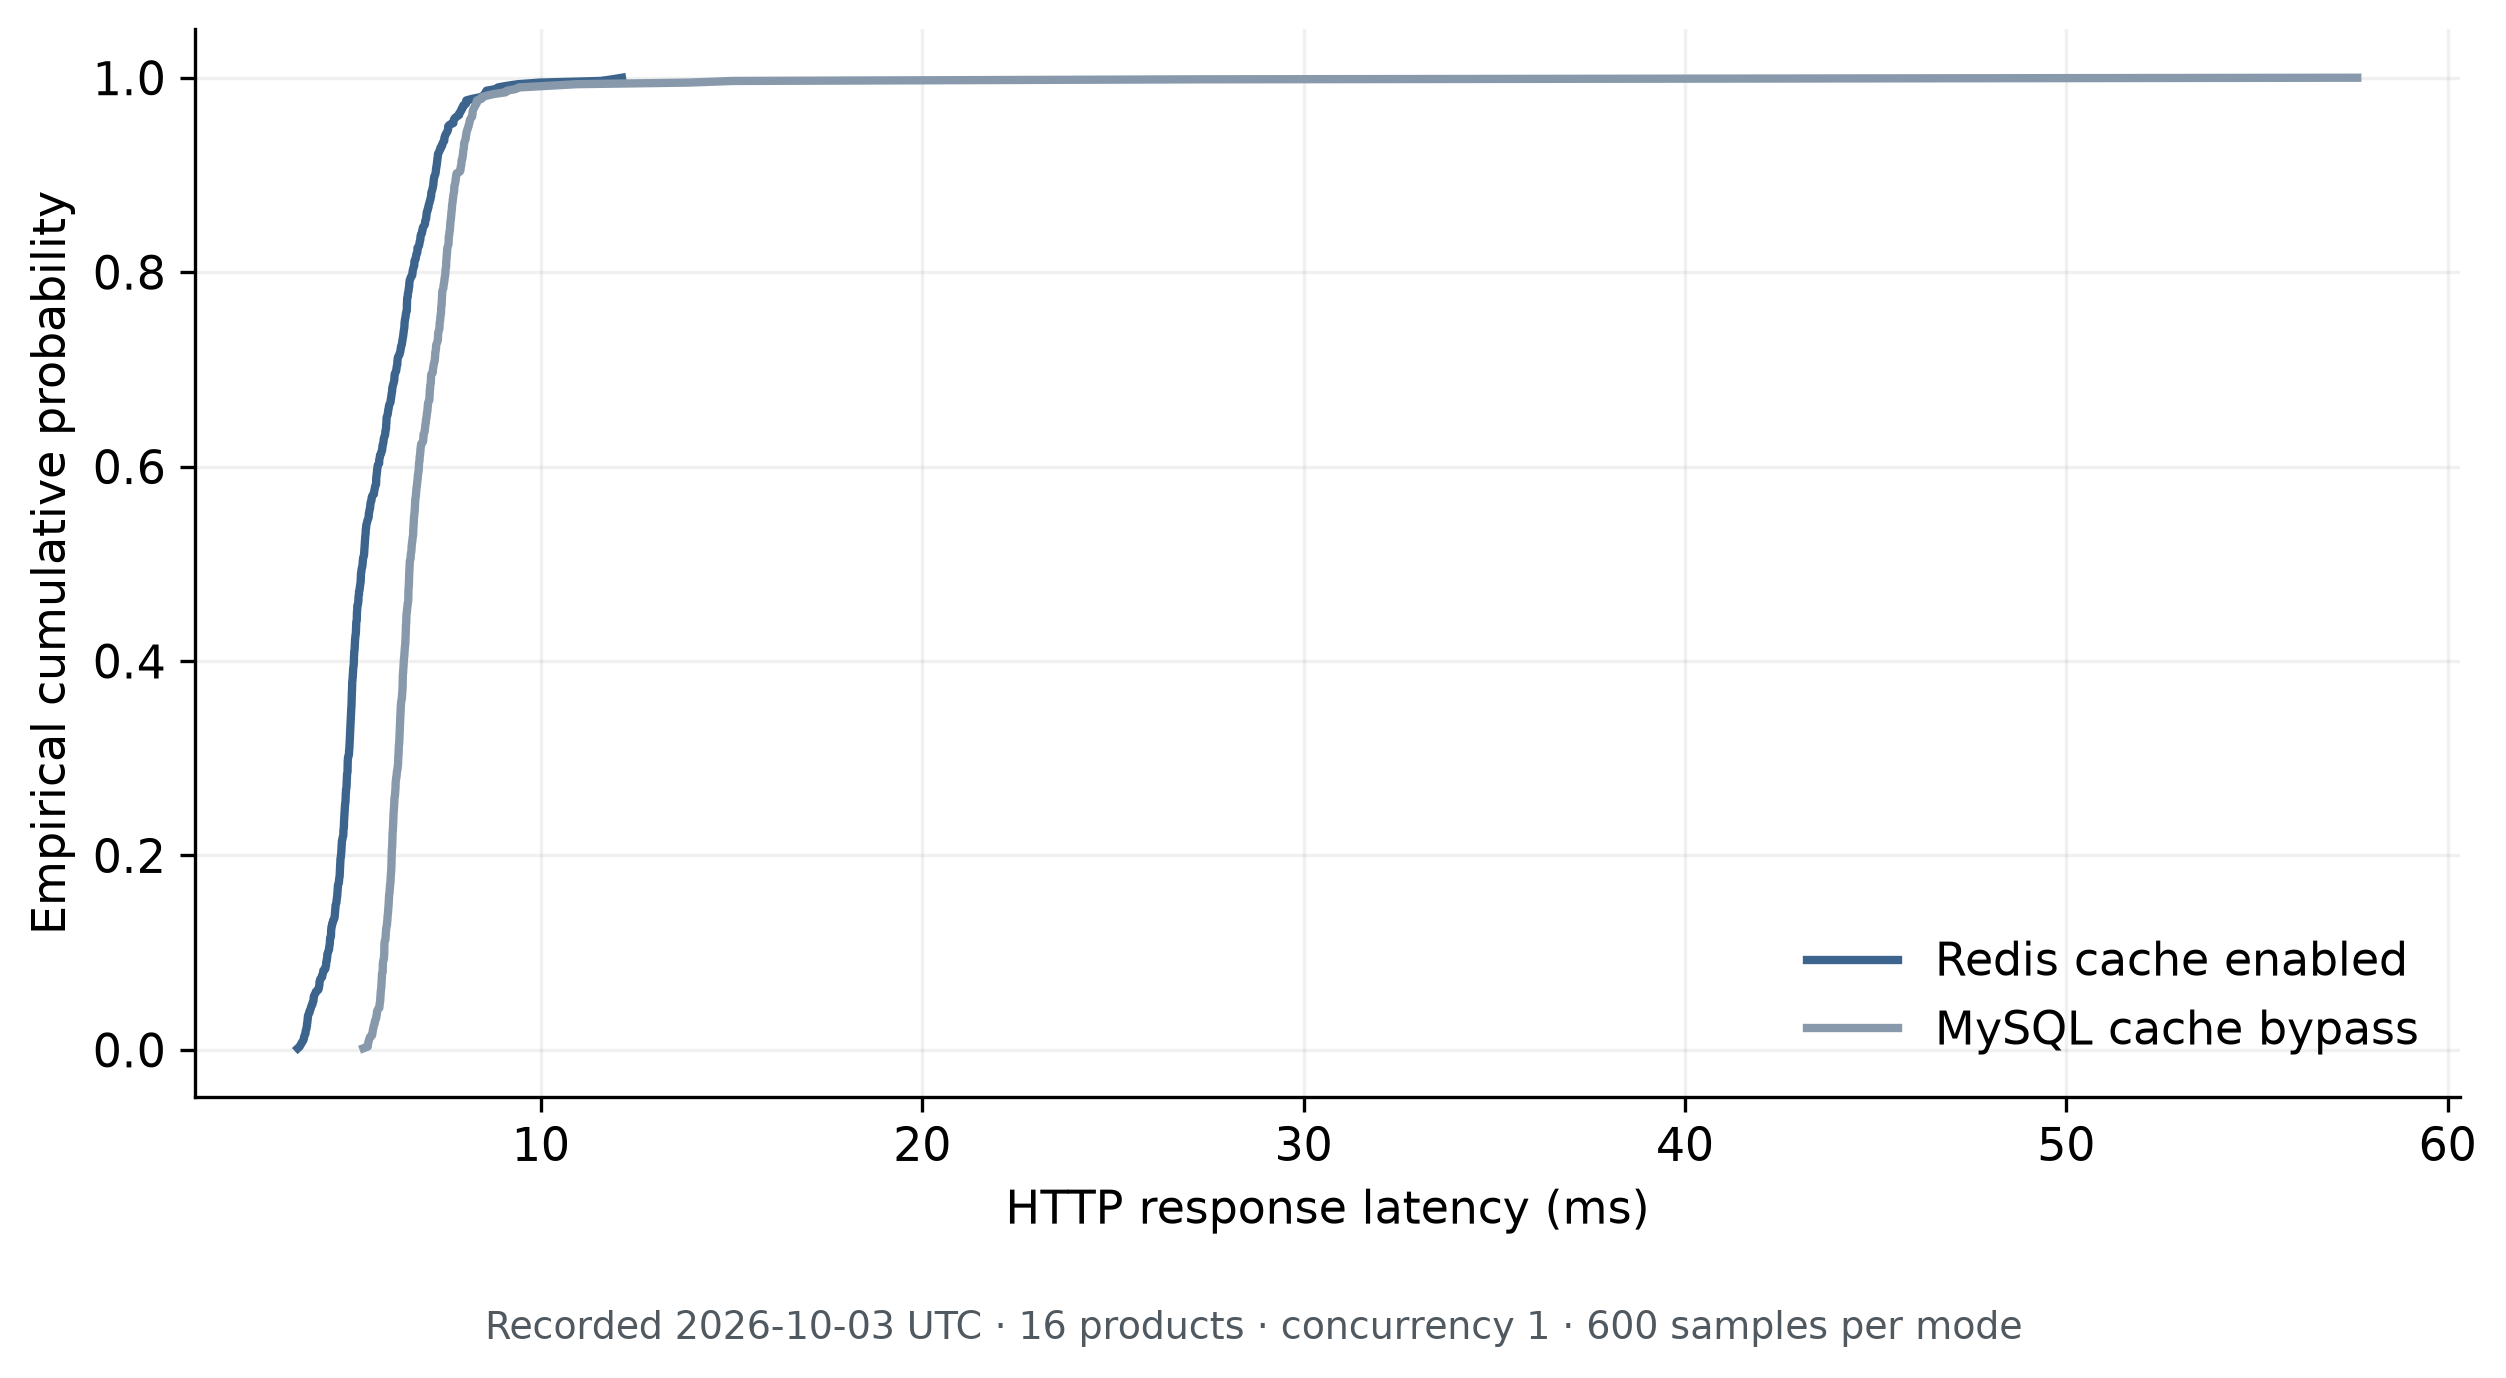
\includegraphics[width=\textwidth,height=0.40\textheight,keepaspectratio]{../figure-assets/evidence/05-latency-ecdf.png}
\caption{Empirical distribution of the preserved warning-query latencies}\label{fig:latency-ecdf}
\end{figure}

The box plot in Figure~\ref{fig:latency-box} shows variability and outlying observations. Those observations should not be silently removed merely to improve the visual result. They also should not be generalized into a production reliability rate. The sample is small in business scope and restricted to one read operation with sequential local traffic.


\begin{figure}[htbp]\centering
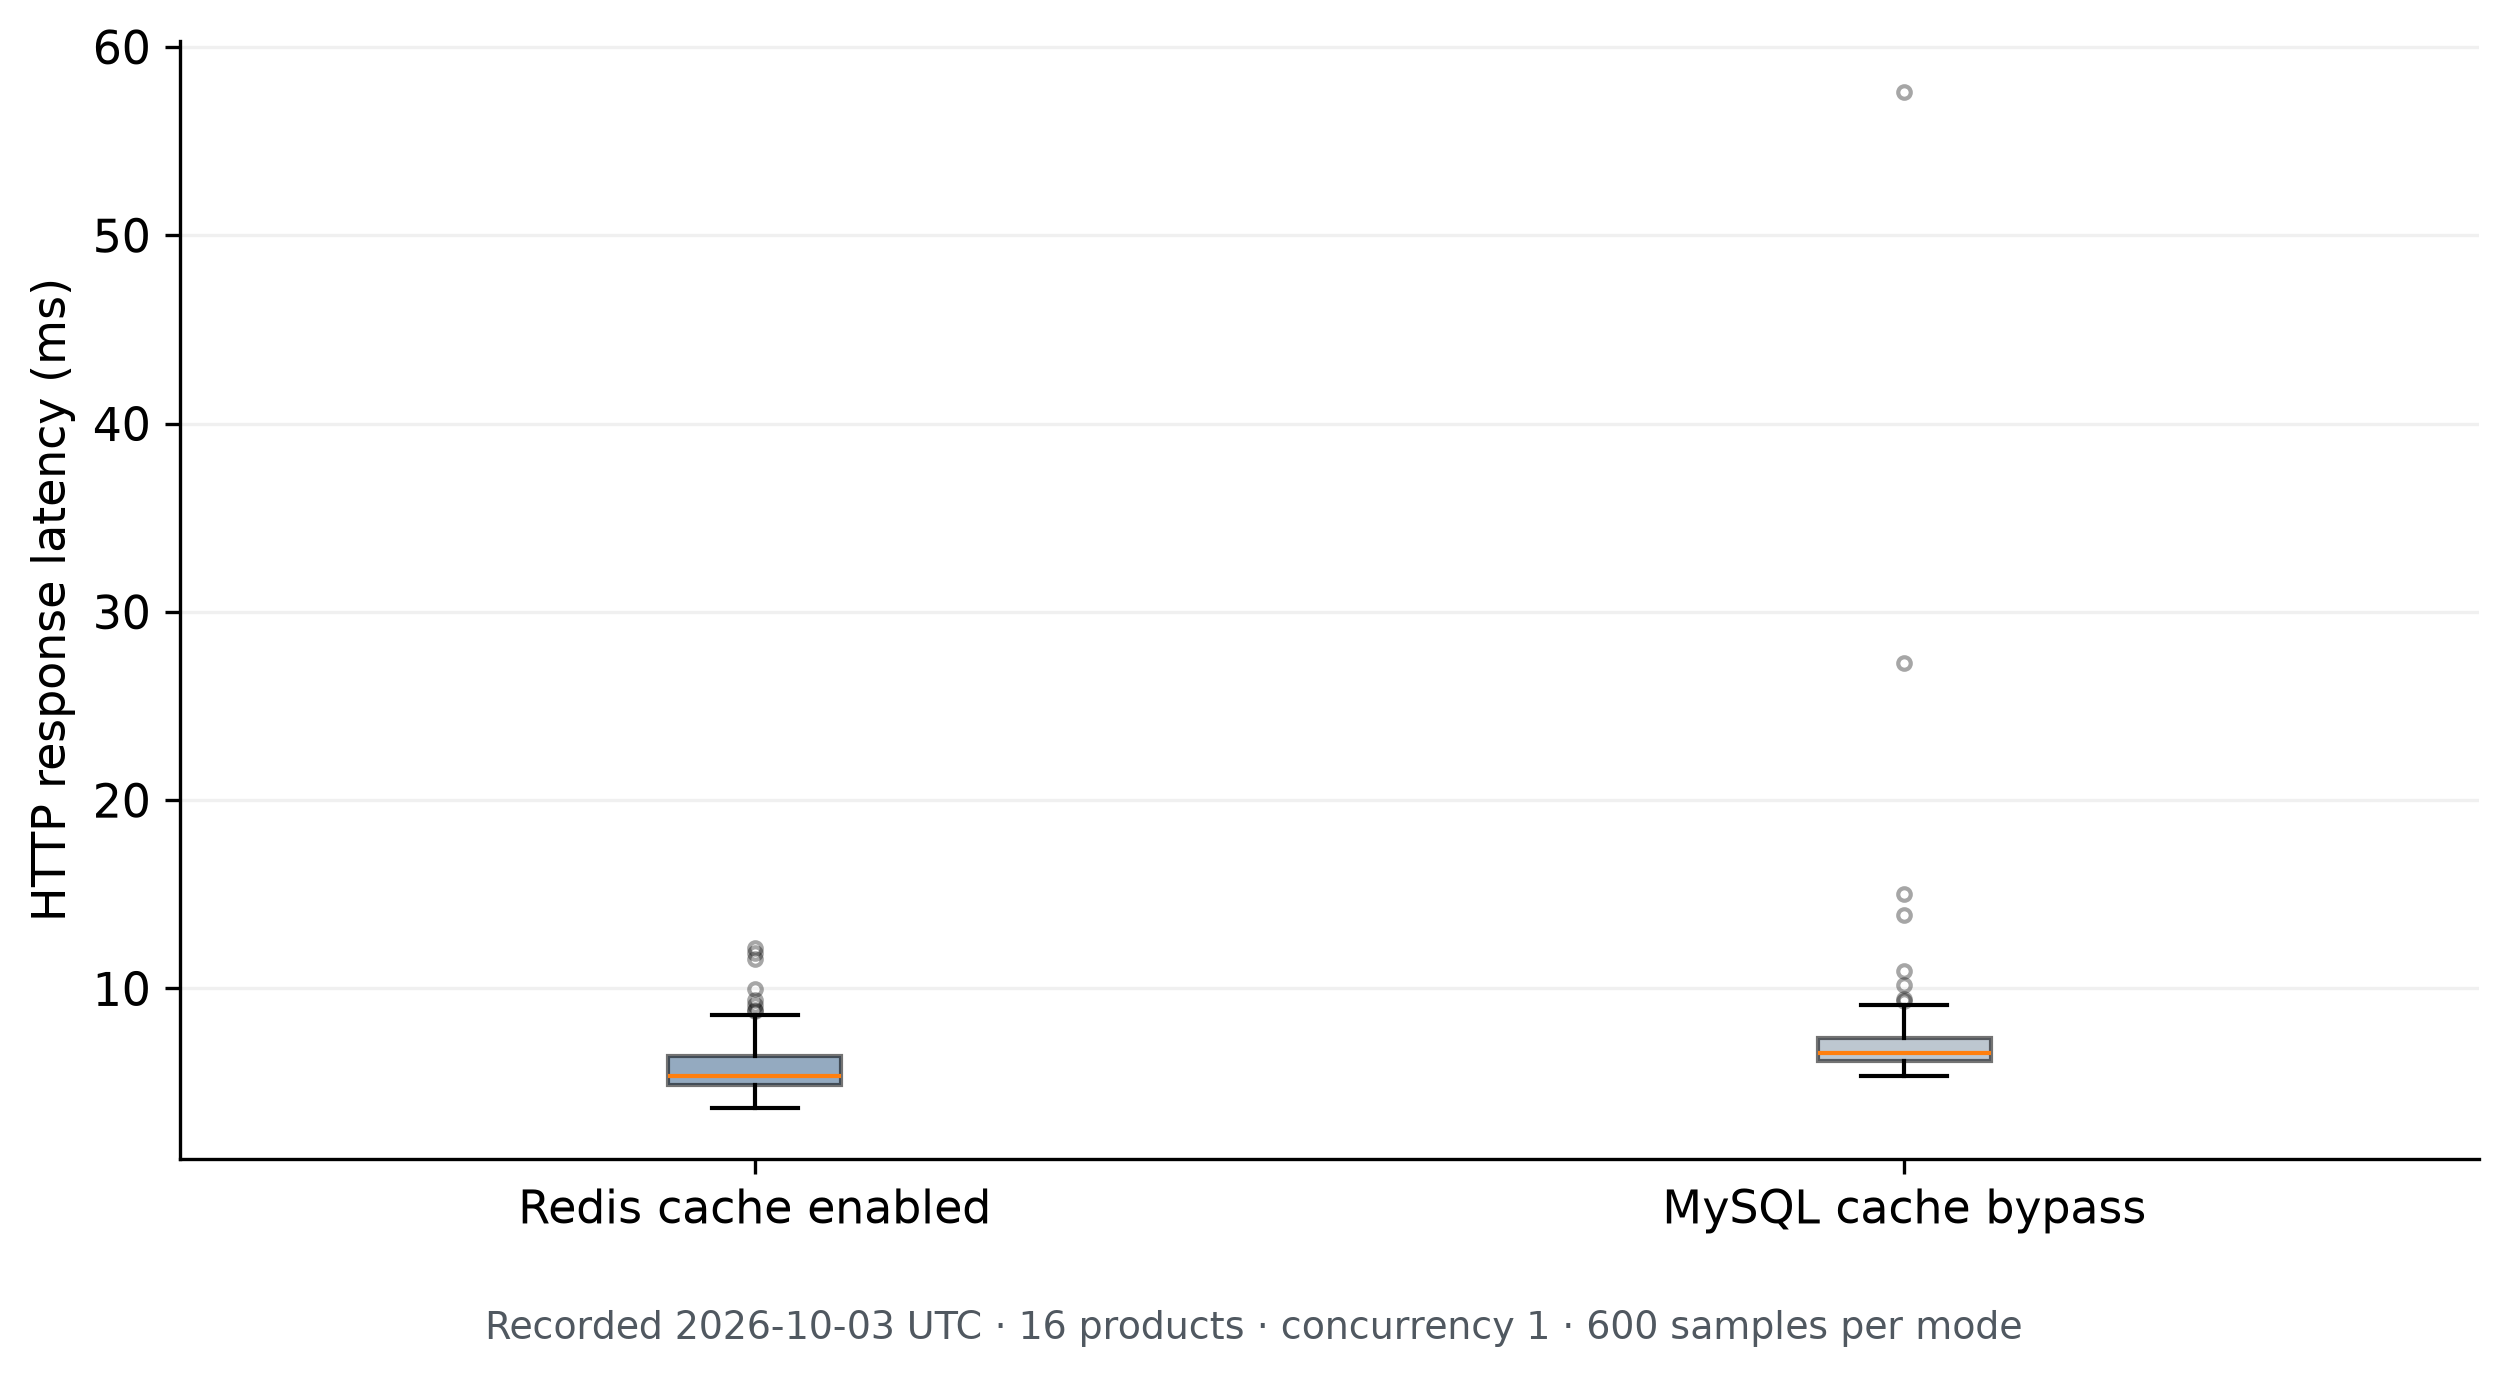
\includegraphics[width=\textwidth,height=0.40\textheight,keepaspectratio]{../figure-assets/evidence/06-latency-boxplot.png}
\caption{Local latency variability including observed outliers}\label{fig:latency-box}
\end{figure}

\FloatBarrier

\subsection{Interpretation and remaining performance work}

The cache reduces repeated page assembly in the tested workload, but each read still obtains a durable revision and checks session authority. A high cache-hit ratio is not equivalent to eliminating database access. The prototype's write path also advances a shared revision row. Testing many writers across different products is therefore a necessary next step before drawing conclusions about larger-store workload behavior.


Useful extensions would vary catalogue size, warning count, page size, concurrent readers and concurrent writers. They would report warm and cold cache behavior, latency distributions, rejected requests and database resource use. A production comparison should control relevant deployment variables and preserve raw samples. These proposed tests describe additional evaluation, not results already obtained.


\FloatBarrier

\section{Recorded failure and persistence checks}

The Redis recovery record stops and restarts only the cache service while MySQL remains available. A cache-enabled query during interruption is compared with the uncached baseline. The record reports the same database warning result during the outage and a recovered service afterward. Individual observed query times are approximately 10.49 ms before interruption, 12.25 ms while unavailable and 25.94 ms after recovery. They are individual observations, not estimates of a recovery-time distribution.


\begingroup\small\setstretch{1.05}\setlength{\tabcolsep}{3pt}\renewcommand{\arraystretch}{1.25}
\begin{longtable}{>{\raggedright\arraybackslash}p{0.3\textwidth}>{\raggedright\arraybackslash}p{0.3\textwidth}>{\raggedright\arraybackslash}p{0.3\textwidth}}
\caption{Recorded cache interruption and restart observations}\label{tab:recovery}\\
\toprule
\textbf{Observation} & \textbf{Recorded result} & \textbf{Supported interpretation} \\
\midrule\endfirsthead
\toprule
\textbf{Observation} & \textbf{Recorded result} & \textbf{Supported interpretation} \\
\midrule\endhead
\bottomrule\endfoot
Redis stopped with MySQL available & Same warning result & Cache outage did not remove authoritative warning data \\
Redis restarted & Recovered service and equivalent result & Normal cache service resumed in this check \\
Application restarted & Same selected stock and movement rows & Durable MySQL state survived ordinary process restart \\
Selected-row fingerprint & 34 rows and equal SHA-256 & Compared product and transaction data remained equal \\
\end{longtable}\endgroup

A separate persistence record compares selected product and transaction rows around an application restart using a fingerprint. It reports equality for thirty-four selected rows. This supports ordinary persistence of those records. It is not a backup restoration, disk-failure or full-database recovery test. Session survival is also a different property: the in-process login state may be lost while stock remains durable.


\FloatBarrier

\section{Traceability and validity of the conclusions}

The acceptance evidence is strongest where a requirement has a direct assertion. Non-negative concurrent stock has a final balance and a success-count check. Exact replay has an identifier and quantity check. Batch allocation has sellable-balance and remainder checks. Purchase approval has recheck, receipt and replay assertions. Acknowledgement and review have reviewer or snapshot checks. Weaker or absent evidence is identified separately, including sustained multi-user workload, external supplier integration and operational usability.


Internal validity is limited by the particular test scenarios and the execution environment. External validity is limited by demonstration data and the single-store boundary. Construct validity depends on using the intended metric: movement counts are not sales, current-price value is not profit, and response latency under one sequential query is not throughput capacity. The thesis maintains those distinctions throughout its figures and result tables.


The current evidence supports a working bounded inventory system with selected consistency and recovery properties. It does not establish a production SLA, a quantified reduction in supermarket stockouts or the safety of unrestricted public deployment. Those conclusions require additional operational controls, workloads and field observations beyond this development study.


\FloatBarrier

\section{Chapter summary}

Functional tests support the implemented stock arithmetic, audit path, role boundaries and selected warning transitions. Browser evidence supports the rendered workflow and selected operational journeys. The local cache benchmark reports a lower pooled median for the enabled path under a small sequential workload. Failure records support cache fallback and ordinary persistence. The following conclusion relates these findings to the original engineering questions and identifies the next work needed for a broader deployment.
